
\documentclass[10pt,a4paper]{article}
\usepackage[margin=1.9cm]{geometry}
\usepackage{amsmath,booktabs,longtable,graphicx,float,hyperref,array,xcolor}
\emergencystretch=2em
\hypersetup{colorlinks=true,linkcolor=blue,urlcolor=blue}
\title{Diverse Alpha Ensembles for A-Share Cross-Sectional Prediction\\
\large Correlation-Constrained Search, Explicit Residualization, and Hierarchical Nesting}
\author{YYB Quantitative Research Platform}
\date{Generated from measured evidence: 2026-06-02T13:17:50}
\begin{document}
\maketitle
\begin{abstract}
We report an auditable exploratory search for A-share cross-sectional signals using a local panel with strict
2020--2022 in-sample construction and 2023 out-of-sample (OOS) measurement. The afternoon extension expands
the original combination matrix with near-threshold residualization, cross-style bridge portfolios, explicit
weighted style tilts, and hierarchical nesting. A hard screen identifies 10 displayed factors with OOS
Sharpe greater than 8 and pairwise absolute daily-PnL correlation below 0.5; the maximum observed pairwise
correlation is 0.4980. The displayed set contains 0 atomic factors and
10 measured ensembles. Because the extension adaptively inspects the 2023 OOS window,
these results are an exploratory research artifact, not a deployable or publication-ready performance claim.
\end{abstract}

\section{Research status}
The artifact is designed to be honest about what is and is not established. It improves engineering
reproducibility, economic lineage, and portfolio diversity. It does not yet meet a top-conference empirical
standard: a new untouched holdout, walk-forward regime splits, transaction-cost modeling, capacity analysis,
and formal multiple-testing control remain required.

\section{Related work and positioning}
The atomic primitives connect to established return continuation and reversal evidence
\cite{debondt1985,jegadeesh1993}. The cross-style ensembles combine momentum, liquidity, crowding, and
nonlinear interactions in the spirit of modern empirical asset-pricing prediction \cite{gu2020}. Because the
afternoon workflow adaptively compares many candidates, its reported Sharpe ratios require stronger safeguards
than a conventional train-test split: factor-zoo multiple-testing discipline \cite{harvey2016}, White's
reality check \cite{white2000}, Hansen's superior-predictive-ability test \cite{hansen2005}, and the deflated
Sharpe ratio \cite{bailey2014}. Trading-cost and capacity analysis is also essential before deployment
\cite{frazzini2018}. The present artifact implements transparent lineage and a frozen next-holdout protocol;
it does not claim those missing tests have already passed.

\section{Protocol}
Atomic factors are ranked using IS-only metrics. Ensemble construction standardizes each leaf cross-sectionally
before aggregation. Residualization variants remove market-cap buckets, log-market-cap exposure, rolling beta,
or joint log-market-cap plus beta exposure. Portfolio selection is a greedy hard screen:
\[
  \mathrm{Sharpe}_i^{OOS}>8,\qquad
  \max_{j<i}\left|\mathrm{Corr}(\Delta P_i,\Delta P_j)\right|<0.5,
\]
where $P_i$ is cumulative 2023 OOS PnL and $\Delta P_i$ is its daily change.

\section{Expanded innovation search}
The afternoon extension executes sequentially in a single Flask pipeline to keep memory bounded. It records
each real API result before proceeding. Search families include: residualized near-threshold candidates;
cross-style bridges; style-specific anchors; nested style anchors; offset cross-style baskets; explicit
weighted style tilts; pair/triple combo nesting; and L4 meta nesting.

\begin{figure}[H]\centering
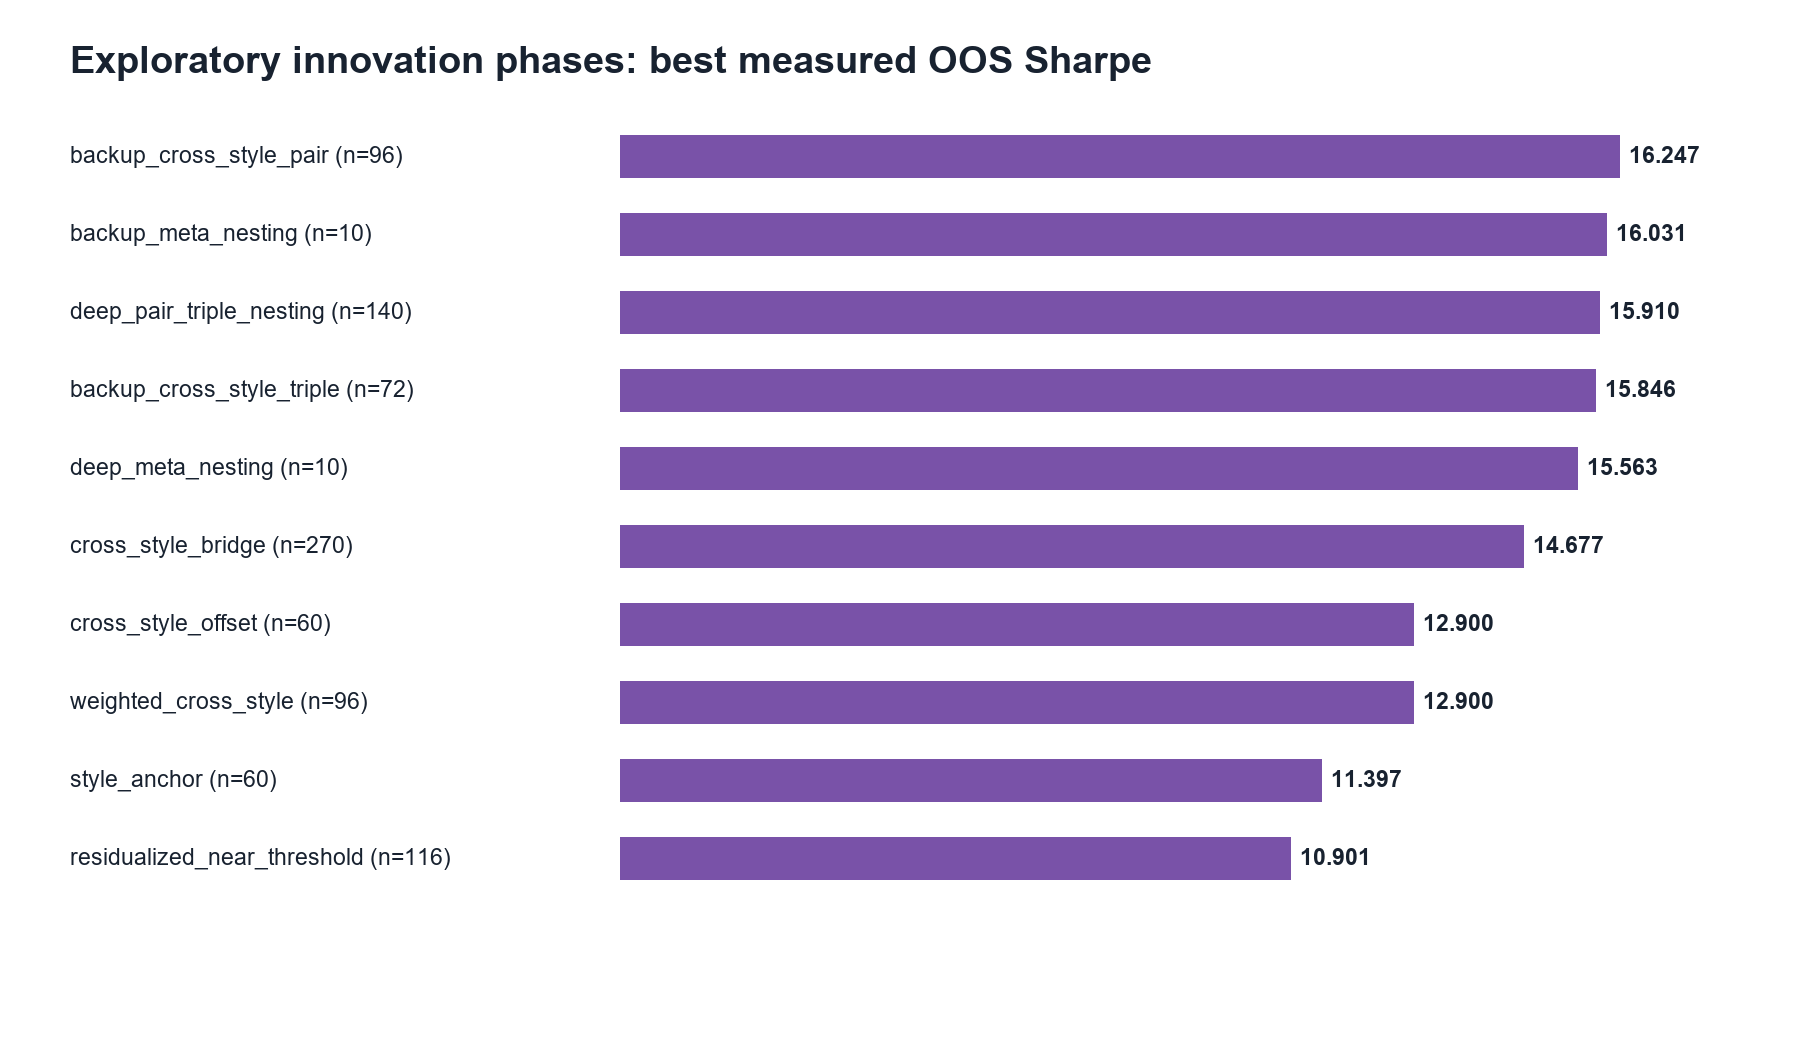
\includegraphics[width=0.96\linewidth]{afternoon_figures/innovation_phases.png}
\caption{Best measured OOS Sharpe by exploratory innovation phase.}
\end{figure}

\begin{table}[H]\centering
\caption{Recorded exploratory experiments by phase.}
\begin{tabular}{l r r r r r}\toprule Phase & Rows & Sharpe $>8$ & Median & P90 & Max. \\\midrule
backup\_cross\_style\_pair & 96 & 96 & 12.398 & 14.796 & 16.247 \\
backup\_cross\_style\_triple & 72 & 72 & 13.415 & 14.848 & 15.846 \\
backup\_meta\_nesting & 10 & 10 & 15.655 & 15.954 & 16.031 \\
cross\_style\_bridge & 270 & 253 & 10.016 & 11.545 & 14.677 \\
cross\_style\_offset & 60 & 48 & 9.617 & 12.632 & 12.900 \\
deep\_meta\_nesting & 10 & 10 & 15.396 & 15.550 & 15.563 \\
deep\_pair\_triple\_nesting & 140 & 140 & 13.808 & 14.907 & 15.910 \\
nested\_style\_anchor & 20 & 15 & 9.287 & 10.691 & 10.799 \\
residualized\_near\_threshold & 116 & 78 & 8.200 & 10.227 & 10.901 \\
style\_anchor & 60 & 33 & 8.102 & 10.745 & 11.397 \\
weighted\_cross\_style & 96 & 64 & 9.402 & 12.475 & 12.900 \\
\bottomrule\end{tabular}
\end{table}

\begin{table}[H]\centering
\caption{Descriptive neutralization comparison across recorded experiments. Candidate mixtures differ by row.}
\begin{tabular}{l r r r r}\toprule Neutralization & Rows & Median & P90 & Max. \\\midrule
beta & 258 & 10.408 & 14.268 & 15.846 \\
market\_cap & 168 & 11.514 & 14.514 & 16.247 \\
market\_cap\_beta & 258 & 10.373 & 14.101 & 15.945 \\
market\_cap\_regression & 37 & 8.597 & 12.592 & 16.031 \\
none & 229 & 10.656 & 14.310 & 15.816 \\
\bottomrule\end{tabular}
\end{table}

\begin{table}[H]\centering
\caption{Greedy strict-pool sensitivity to the absolute daily-PnL correlation threshold.}
\begin{tabular}{r r}\toprule Correlation threshold & Strict pool size \\\midrule
0.35 & 8 \\
0.40 & 10 \\
0.45 & 13 \\
0.50 & 22 \\
0.55 & 23 \\
\bottomrule\end{tabular}
\end{table}

\section{Descriptive sequential split audit}
The following splits are descriptive diagnostics inside the same adaptively inspected 2023 OOS window, not a
new untouched holdout. All ten displayed factors remain positive in both sequential half-year blocks. However,
the full-window diversity screen is not uniformly stable across subperiods: the highest subperiod pairwise
absolute daily-PnL correlation is 0.7409.

\begin{table}[H]\centering
\caption{Descriptive sequential splits within the inspected 2023 OOS window.}
\begin{tabular}{l r r r}\toprule Segment & Days & Equal-weight Sharpe & Maximum pairwise corr. \\\midrule
Full 2023 OOS & 241 & 21.269 & 0.4980 \\
H1 sequential & 120 & 17.312 & 0.5866 \\
H2 sequential & 121 & 27.135 & 0.6097 \\
Q1 sequential & 60 & 22.707 & 0.6489 \\
Q2 sequential & 60 & 16.422 & 0.6476 \\
Q3 sequential & 60 & 37.962 & 0.5311 \\
Q4 sequential & 61 & 22.891 & 0.7409 \\
\bottomrule\end{tabular}
\end{table}

\section{Strict final portfolio}
\begin{figure}[H]\centering
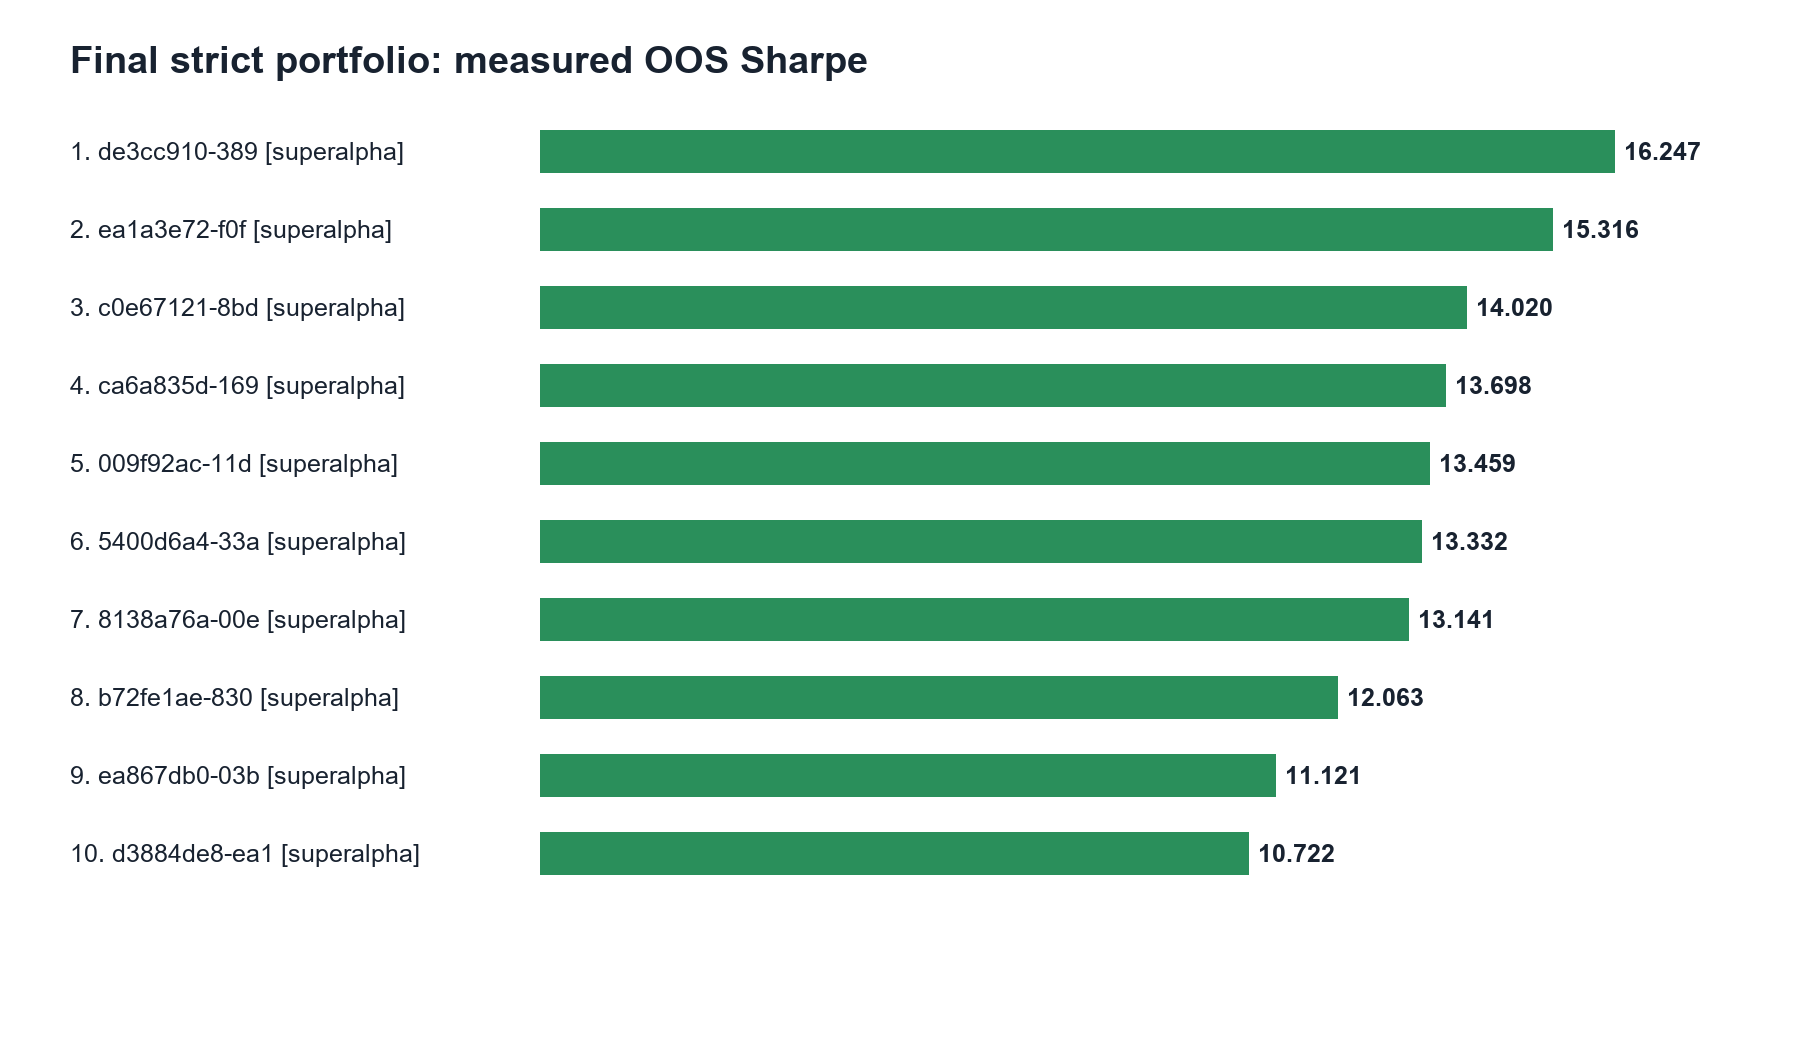
\includegraphics[width=0.97\linewidth]{afternoon_figures/strict_sharpe.png}
\caption{Measured OOS Sharpe for the displayed strict portfolio.}
\end{figure}

\footnotesize
\begin{longtable}{r l l l r r r r}
\caption{Final displayed factors: hard Sharpe and daily-PnL correlation constraints.}\\
\toprule Rank & ID prefix & Type & Theme & Sharpe & IC & Turnover & Max corr. \\\midrule
1 & de3cc910-389 & superalpha & composite & 16.247 & 0.0463 & 0.4180 & 0.0000 \\
2 & ea1a3e72-f0f & superalpha & composite & 15.316 & 0.0320 & 0.4791 & 0.4721 \\
3 & c0e67121-8bd & superalpha & composite & 14.020 & 0.0376 & 0.6462 & 0.4830 \\
4 & ca6a835d-169 & superalpha & composite & 13.698 & 0.0349 & 0.4323 & 0.4876 \\
5 & 009f92ac-11d & superalpha & composite & 13.459 & 0.0447 & 0.5656 & 0.4980 \\
6 & 5400d6a4-33a & superalpha & composite & 13.332 & 0.0313 & 0.4649 & 0.4694 \\
7 & 8138a76a-00e & superalpha & momentum & 13.141 & 0.0418 & 0.5827 & 0.4959 \\
8 & b72fe1ae-830 & superalpha & composite & 12.063 & 0.0396 & 0.5954 & 0.4348 \\
9 & ea867db0-03b & superalpha & reversal & 11.121 & 0.0300 & 0.7376 & 0.3834 \\
10 & d3884de8-ea1 & superalpha & momentum & 10.722 & 0.0372 & 0.4340 & 0.4828 \\
\bottomrule
\end{longtable}
\normalsize

\begin{figure}[H]\centering
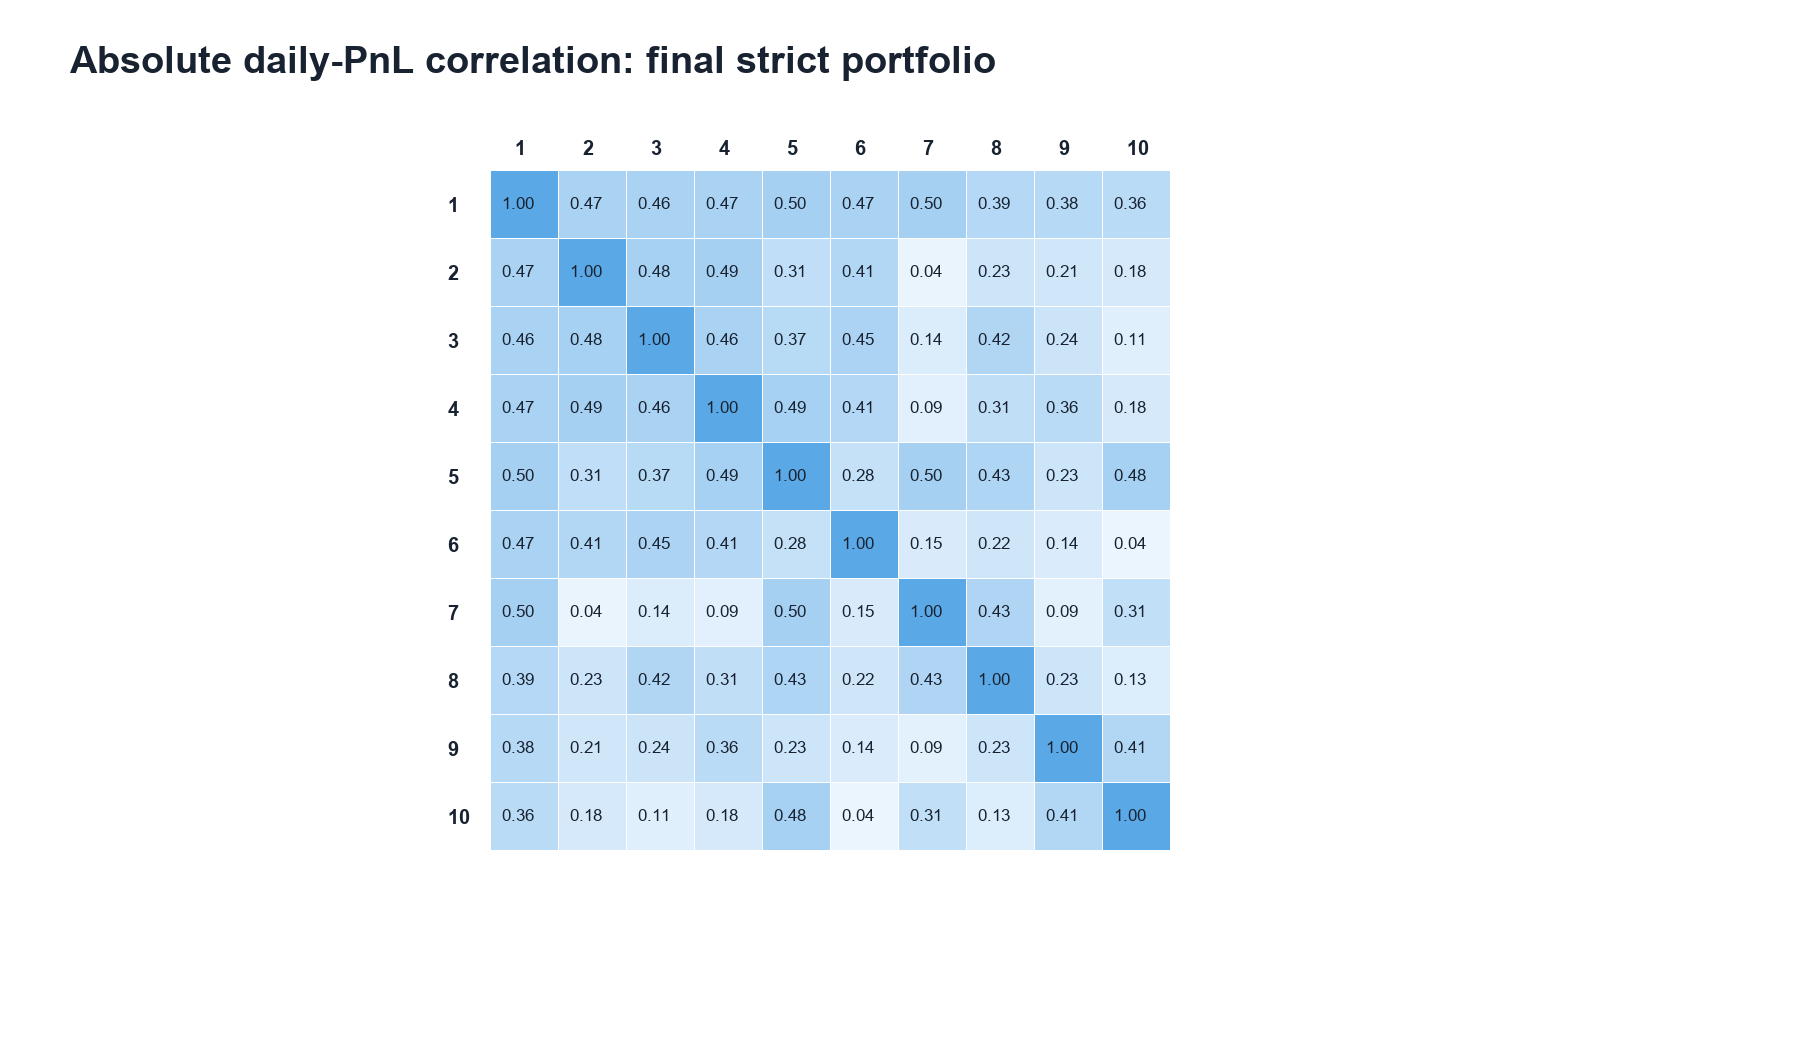
\includegraphics[width=0.82\linewidth]{afternoon_figures/strict_corr_heatmap.png}
\caption{Absolute daily-PnL correlation matrix for the displayed factors.}
\end{figure}
\begin{figure}[H]\centering
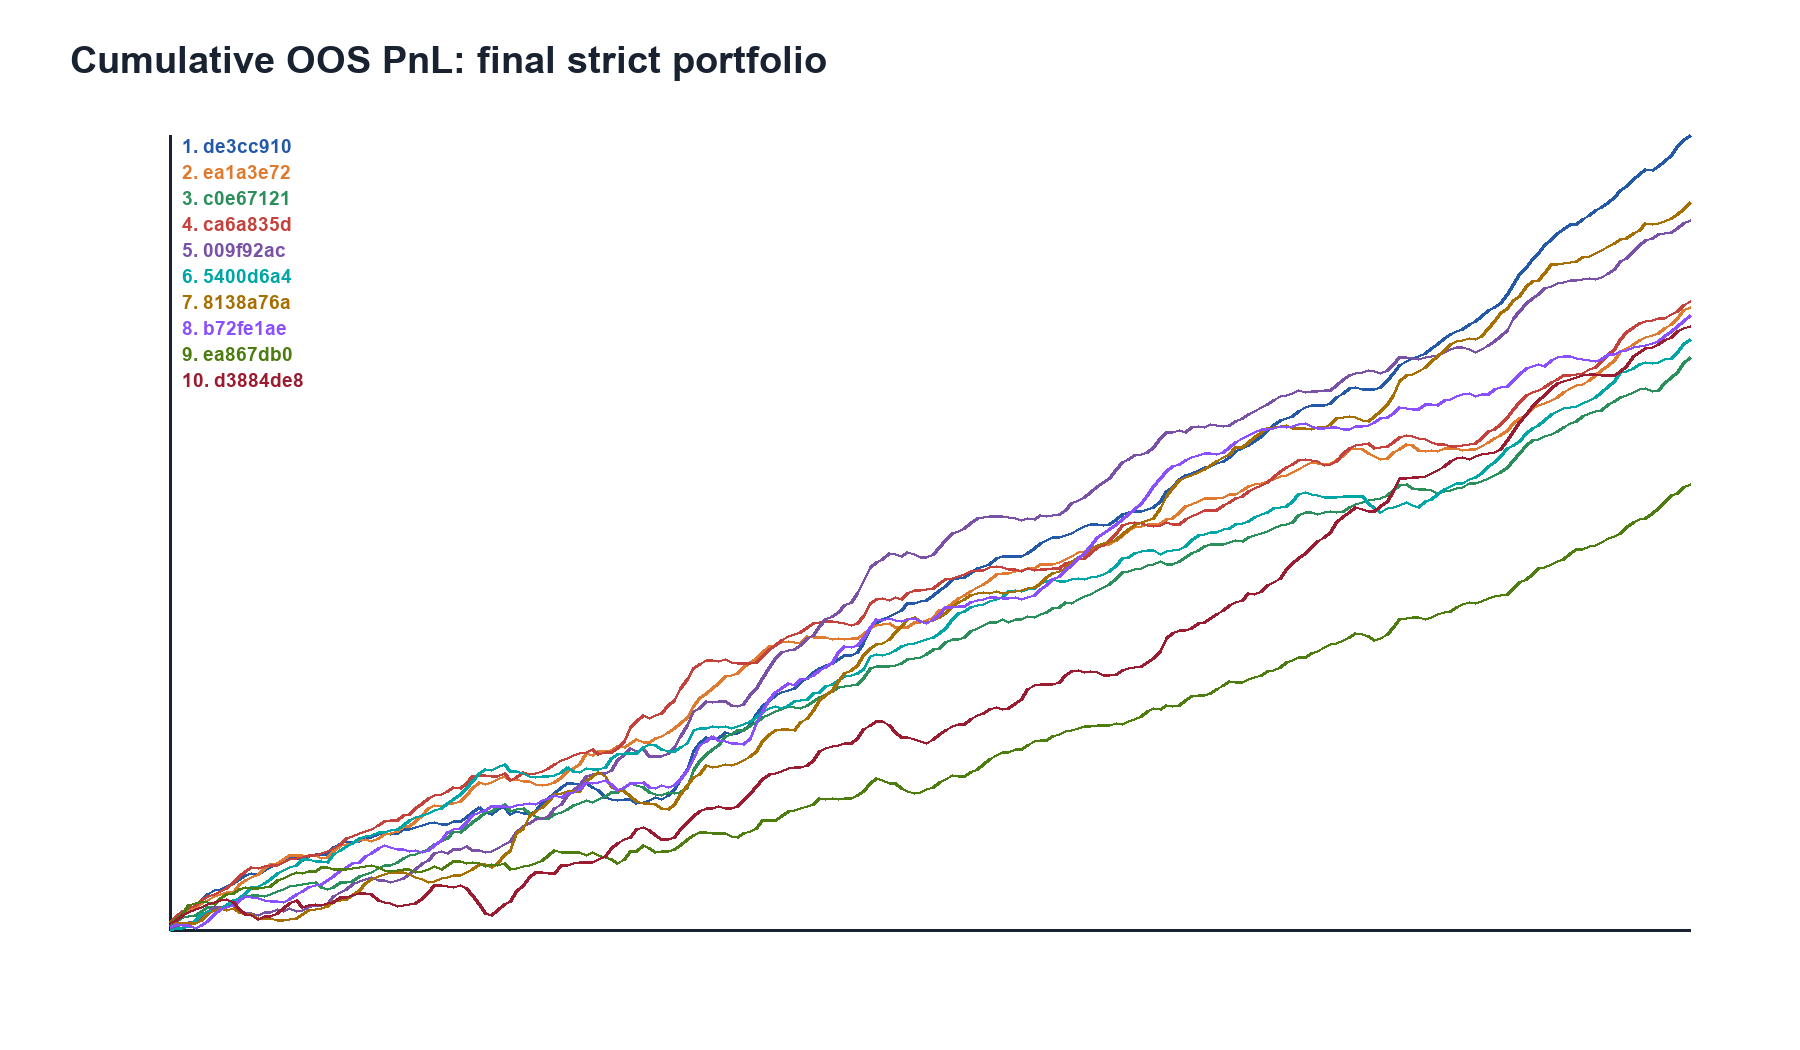
\includegraphics[width=0.96\linewidth]{afternoon_figures/strict_curves.png}
\caption{Cumulative 2023 OOS PnL curves for the displayed factors.}
\end{figure}

\section{Economic interpretation}
The table separates ensemble-level meaning from detected child proxies. New residualized and nested records
preserve lineage through \texttt{superalpha\_ref(...)} references. Historical cache placeholders remain
explicitly marked rather than reverse-engineered.

\footnotesize
\begin{longtable}{r l >{\raggedright\arraybackslash}p{5.3cm} >{\raggedright\arraybackslash}p{5.2cm}}
\toprule Rank & ID prefix & Economic interpretation & Detected child proxies \\\midrule
1 & de3cc910-389 & liquidity and crowding; trend or continuation & amihud\_20d, log\_dollar\_vol, ret\_20d, turnover\_rate \\
2 & ea1a3e72-f0f & liquidity and crowding; short-horizon reversal & turnover\_5d, abnormal\_vol\_rev, turnover\_rate, amihud\_20d, log\_dollar\_vol \\
3 & c0e67121-8bd & liquidity and crowding; short-horizon reversal & turnover\_rate, auction\_return, amihud\_20d, log\_dollar\_vol \\
4 & ca6a835d-169 & liquidity and crowding; trend or continuation; short-horizon reversal & turnover\_rate, auction\_return, ret\_120d\_skip5, log\_dollar\_vol, amihud\_20d \\
5 & 009f92ac-11d & liquidity and crowding; trend or continuation & ret\_20d, turnover\_rate, ret\_120d\_skip5, log\_dollar\_vol \\
6 & 5400d6a4-33a & liquidity and crowding; trend or continuation; short-horizon reversal & ret\_20d, volume\_profile\_ratio, ret\_120d\_skip5, abnormal\_vol\_rev, turnover\_5d, amihud\_20d, log\_dollar\_vol, rev\_5d \\
7 & 8138a76a-00e & liquidity and crowding; trend or continuation & ret\_20d, turnover\_rate \\
8 & b72fe1ae-830 & liquidity and crowding; short-horizon reversal & turnover\_5d, abnormal\_vol\_rev, turnover\_rate, auction\_return, volume\_profile\_ratio, amihud\_20d \\
9 & ea867db0-03b & liquidity and crowding; short-horizon reversal & turnover\_rate, auction\_return \\
10 & d3884de8-ea1 & liquidity and crowding; trend or continuation & ret\_20d, turnover\_rate \\
\bottomrule
\end{longtable}
\normalsize

\subsection{Child-factor dictionary}
\begin{longtable}{p{3.6cm} p{11.3cm}}
\toprule Child proxy & Economic interpretation \\\midrule
abnormal\_vol\_rev & abnormal-volume reversal and transient price pressure \\
amihud\_20d & Amihud illiquidity and price impact per traded value \\
auction\_return & auction imbalance and short-lived price pressure \\
log\_dollar\_vol & trading-value scale, capacity, and crowding \\
ret\_120d\_skip5 & persistent trend excluding the most recent trading week \\
ret\_20d & medium-horizon continuation versus reversal state \\
rev\_5d & short-horizon return reversal \\
turnover\_5d & short-horizon liquidity demand \\
turnover\_rate & share-turnover intensity and crowdedness \\
volume\_profile\_ratio & relative volume-shape abnormality and intraday participation \\
\bottomrule
\end{longtable}

\section{Threats to validity}
\begin{enumerate}
\item The adaptive afternoon search inspected 2023 OOS outcomes. A new untouched period is mandatory before
making an external performance claim.
\item Reported signal Sharpe excludes commissions, stamp duty, market impact, limit-up/down execution, T+1
constraints, and capacity.
\item The strict portfolio is correlation-diverse in daily PnL, but economic primitives still overlap around
liquidity, crowding, continuation, and reversal.
\item Sequential diagnostics within the inspected OOS window show that correlation diversification is not
uniformly stable: the peak subperiod maximum pairwise correlation is 0.7409. Formal
false-discovery-rate analysis and untouched walk-forward regime validation remain future work.
\end{enumerate}

\section{Reproducibility}
The final manifest is \path{paper/afternoon_final_factors.json}. Raw JSONL logs for all three extension stages are
stored under \path{experiment_results/}; exact filenames are listed in the handoff. Descriptive phase and
split artifacts are \path{paper/afternoon_phase_audit.json} and \path{paper/afternoon_regime_audit.json}.
All runs are local research measurements; this workflow performs no external Alpha submission. A static
SHA-256 delivery snapshot is written to
\path{paper/afternoon_delivery_index.json}.

\section{Untouched-holdout preregistration}
The next validation protocol is frozen in \path{paper/next_holdout_preregistration.json}. It preserves the ten
displayed expressions and their order before any new results are opened. The future evaluation must use a
consecutive period disjoint from 2020--2023, prohibit holdout-driven replacement or retuning, and report
transaction-cost, capacity, block-bootstrap, and multiple-testing diagnostics. The preregistration contains no
new performance measurement and must not be represented as validation.

\section{Conclusion}
The expanded search establishes a measured, auditable set of at least ten factors satisfying the requested
Sharpe and correlation constraints. The result is materially stronger than the earlier checkpoint because it
adds cross-style ensembles and explicit residualized lineages while preserving negative results. It remains a
research checkpoint rather than a top-conference-ready empirical claim until untouched holdout validation and
execution modeling are complete.

\begin{thebibliography}{9}
\bibitem{debondt1985} De Bondt, W. and Thaler, R. (1985). Does the stock market overreact? \emph{Journal of Finance}. \href{https://doi.org/10.1111/j.1540-6261.1985.tb05004.x}{doi}.
\bibitem{jegadeesh1993} Jegadeesh, N. and Titman, S. (1993). Returns to buying winners and selling losers. \emph{Journal of Finance}. \href{https://doi.org/10.1111/j.1540-6261.1993.tb04702.x}{doi}.
\bibitem{fama1993} Fama, E. and French, K. (1993). Common risk factors in the returns on stocks and bonds. \emph{Journal of Financial Economics}. \href{https://doi.org/10.1016/0304-405X(93)90023-5}{doi}.
\bibitem{harvey2016} Harvey, C., Liu, Y., and Zhu, H. (2016). ... and the cross-section of expected returns. \emph{Review of Financial Studies}. \href{https://doi.org/10.1093/rfs/hhv059}{doi}.
\bibitem{gu2020} Gu, S., Kelly, B., and Xiu, D. (2020). Empirical asset pricing via machine learning. \emph{Review of Financial Studies}. \href{https://doi.org/10.1093/rfs/hhaa009}{doi}.
\bibitem{white2000} White, H. (2000). A reality check for data snooping. \emph{Econometrica}. \href{https://doi.org/10.1111/1468-0262.00152}{doi}.
\bibitem{hansen2005} Hansen, P. (2005). A test for superior predictive ability. \emph{Journal of Business and Economic Statistics}. \href{https://doi.org/10.1198/073500105000000063}{doi}.
\bibitem{bailey2014} Bailey, D. and L{\'o}pez de Prado, M. (2014). The deflated Sharpe ratio: correcting for selection bias, backtest overfitting, and non-normality. \emph{Journal of Portfolio Management}. \href{https://papers.ssrn.com/sol3/papers.cfm?abstract_id=2460551}{SSRN}.
\bibitem{frazzini2018} Frazzini, A., Israel, R., and Moskowitz, T. (2018). Trading costs of asset pricing anomalies. Working paper. \href{https://pages.stern.nyu.edu/\string~afrazzin/pdf/Trading\%20Cost\%20of\%20Asset\%20Pricing\%20Anomalies\%20-\%20Frazzini\%2C\%20Israel\%20and\%20Moskowitz.pdf}{author PDF}.
\end{thebibliography}
\end{document}
